% The estimation-to-design loop, closed. Authored 2026-09-15 for Lecture 8,
% answering two notes on Alex's annotated build: "yes, we should draw the loop"
% (beside the future-work figure note on 8-9) and item 4 of his major feedback,
% where he drew the cycle himself as
%     digital experiment -> PE -> DoE -> (arrow back to digital experiment).
%
% WHAT THE FIGURE MUST CARRY. The lecture's thesis is that the SAME matrix is
% computed twice for two different purposes: estimation produces Q and reads M
% to report uncertainty; design writes M to choose the next experiment. So the
% FIM sits in the middle, touched by both arcs, rather than living inside one
% box. Everything else is a stage of the loop.
%
% The "digital experiment" box is drawn dashed on purpose: in the course
% notebook it is simulation standing in for a laboratory, and a student should
% not come away thinking the loop requires a simulator. Replace that one box
% with a real instrument and nothing else in the diagram changes.
%
% GREYSCALE. Okabe-Ito blue #0072B2 for the two optimization problems, orange
% #E69F00 for the FIM at the centre. Nothing is carried by colour: the two
% optimization boxes are rounded, the experiment boxes are sharp, the simulated
% one is dashed, and every arrow is labelled with what travels along it.
%
% TIKZ LIBRARIES. arrows.meta and positioning, both loaded by the pack preamble.

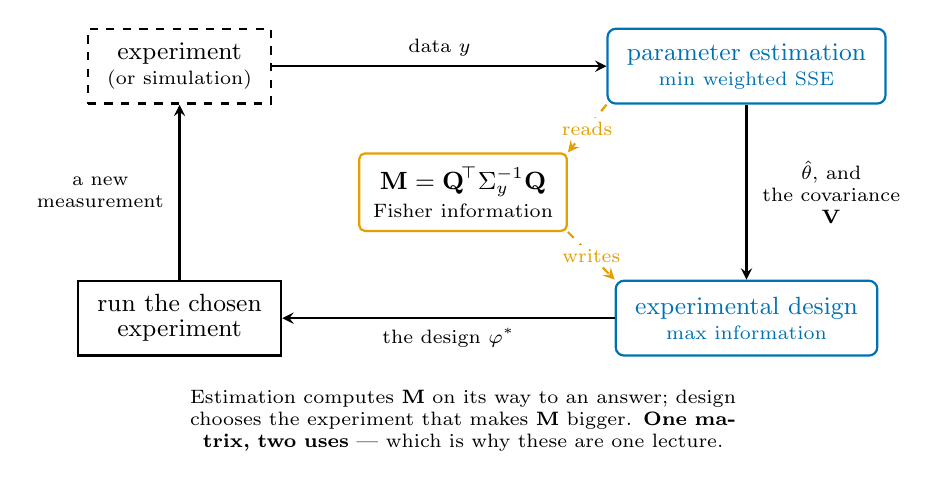
\begin{tikzpicture}[
  font=\small, >=stealth,
  opt/.style={draw, thick, rounded corners=3pt, align=center,
              minimum height=0.95cm, inner xsep=7pt, draw=loopblue, text=loopblue},
  expt/.style={draw, thick, align=center, minimum height=0.95cm, inner xsep=7pt},
  lbl/.style={font=\scriptsize, align=center}
]
  \definecolor{loopblue}{HTML}{0072B2}
  \definecolor{looporange}{HTML}{E69F00}

  % --- the four stations, clockwise from top left ---------------------------
  \node[expt, dashed] (expt) at (-3.6, 1.6)
    {experiment\\[-2pt]{\scriptsize (or simulation)}};
  \node[opt]          (pe)   at ( 3.6, 1.6)
    {parameter estimation\\[-2pt]{\scriptsize $\min$ weighted SSE}};
  \node[opt]          (doe)  at ( 3.6,-1.6)
    {experimental design\\[-2pt]{\scriptsize $\max$ information}};
  \node[expt]         (next) at (-3.6,-1.6)
    {run the chosen\\[-2pt]experiment};

  % --- the FIM at the centre, touched by both arcs --------------------------
  \node[draw, thick, fill=white, draw=looporange, rounded corners=2pt,
        align=center, inner sep=5pt] (fim) at (0,0)
    {$\mathbf{M} = \mathbf{Q}^{\!\top}\boldsymbol{\Sigma}_y^{-1}\mathbf{Q}$\\[-1pt]
     {\scriptsize Fisher information}};

  % --- the loop -------------------------------------------------------------
  \draw[->, thick] (expt) -- (pe) node[lbl, midway, above] {data $y$};
  \draw[->, thick] (pe)   -- (doe)
    node[lbl, midway, right, xshift=2pt] {$\hat{\theta}$, and\\ the covariance\\ $\mathbf{V}$};
  \draw[->, thick] (doe)  -- (next)
    node[lbl, midway, below] {the design $\varphi^{*}$};
  \draw[->, thick] (next) -- (expt)
    node[lbl, midway, left, xshift=-2pt] {a new\\ measurement};

  % --- both arcs touch the same matrix --------------------------------------
  % Labels sit BELOW/ABOVE their midpoints and are pulled toward the centre:
  % first render put "reads" on the PE box's bottom rule and "writes" on the
  % DoE box's top rule. Caught by looking at the page, not by compiling.
  \draw[->, looporange, thick, dashed] (pe.south west) -- (fim.north east)
    node[lbl, pos=0.5, fill=white, inner sep=1.5pt, text=looporange] {reads};
  \draw[->, looporange, thick, dashed] (fim.south east) -- (doe.north west)
    node[lbl, pos=0.5, fill=white, inner sep=1.5pt, text=looporange] {writes};

  \node[lbl, text width=8.6cm] at (0,-2.9)
    {Estimation computes $\mathbf{M}$ on its way to an answer; design chooses
     the experiment that makes $\mathbf{M}$ bigger. \textbf{One matrix, two
     uses} --- which is why these are one lecture.};
\end{tikzpicture}
